% LaTeX .tex
% Example for the proceedings of the  25th International Congress of Mechanical Engineering
% COBEM 2019
% October, 20-25, 2019, Uberlândia, MG, Brazil
% Based on the template of the proceedings of COBEM2015 and COBEM2017

\documentclass[10pt,fleqn,a4paper,twoside]{article}
\usepackage{abcm}
\def\shortauthor{M. F. O. Miranda, F. J. O. Ribeiro, N. S. Saad and A. Z. Guarato}
\def\shorttitle{Experimental Analysis on the Mechanical Properties of Fused Deposition Modeling Parts}
\usepackage{subcaption}
\captionsetup{compatibility=false}
\usepackage{blindtext}
\begin{document}
\fphead
\hspace*{-2.5mm}\begin{tabular}{||p{\textwidth}}
\begin{center}
\vspace{-4mm}
\title{EXPERIMENTAL ANALYSIS ON THE MECHANICAL PROPERTIES OF PETG PARTS MADE WITH FUSED DEPOSITION MODELING MANUFACTURING}
\end{center}
\authors{Ma\'ira Fernanda Oliveira de Miranda} \\
\authors{Felipe Jose Oliveira Ribeiro} \\
\institution{Federal University of Uberl\^andia (UFU), Av. Jo\~ao Naves de \'Avila, 2121, Campos Santa M\^onica, Uberl\^andia, MG } \\
\institution{mairaf\_miranda@hotmail.com} \\
\institution{feliperibeiro.ufu@gmail.com} \\
\vspace{0.5mm}
\authors{Núbia dos Santos Saad}\\
\authors{Alexandre Zuquete Guarato}\\
\institution{Federal University of Uberl\^andia (UFU), Av. Jo\~ao Naves de \'Avila, 2121, Campos Santa M\^onica, Uberl\^andia, MG } \\
\institution{nubia@ufu.br}\\
\institution{azguarato@ufu.br} \\
\\
\abstract{\textbf{Abstract.}  Fast prototyping technology, especially 3D printing, has been gaining increasing importance for its suitability and constant decrease of costs in printing equipment and material. In the present paper, the authors study the mechanical properties of parts made with the fusion deposition modeling process. The material used was the PETG XT from 3DFila. It was studied the variation of the mechanical properties in function of the temperature of extrusion. The temperatures studied were 230 $^\circ C$, 240 $^\circ C$, 245 $^\circ C$ and 250 $^\circ C$, with five test bodies made for each temperature. The specimens were made solid, with 100\% infill and according geometrically with the ASTM D638-02a standard. Then tensile tests were performed in each one of the twenty test parts in order to observe the Young's modulus that prevail in each temperature. The results were then compared with literature. It was observed that the elasticity coefficient increased with the temperature on the hot end.}\\
\\
\keywords{\textbf{Keywords:} FDM(Fused Deposition Modeling), PETG(Polyethylene Terephthalate Glycol), Young modulus, Poisson coefficient, Stress test }\\
\end{tabular}



\section{INTRODUCTION}

The fusion deposition modeling process is a manufacturing methodology ideal for prototyping. Because of its automation, there is a relatively simple setup that has to be done, and with some practice it becomes simple to develop complex mechanical geometries \citep{fdm_today},\citep{metal_dental_implants}, some of which even being impossible to be made from other classic manufacturing processes.   

PETG (Polyethylene Terephthalate Glycol) is a polymer that has been steadily gaining popularity among the 3D printing community, since it combines the reliability of PLA (polylactic acid), in terms of overall easy printability, with the durability of ABS (Acrylonitrile Butadiene Styrene), in terms of mechanical resilience properties \citep{tiposfilamento}. Such fact makes this polymer a good choice when prototyping mechanical parts. It is also worth mentioning that the PETG deforms much more than ABS before breaking, making this material better suited for critical structural applications. 

But, even though there are advantages, when it comes to the finished printed parts, there are some complications in the usability of the material \citep{3Dcomplication}: Since 3D printing is not yet well standardized by the manufacturers, it is impossible to safely predict the final properties of the parts because there are many parameters that influence the printing part of the process, such as printing temperature, rate, geometry, infill percentage \citep{infill}, temperature of the printing surface \citep{temp_mesa} and nozzle width \citep{ABS_PLA_today}. Another problem is that the final FDM part also becomes anisotropic \citep{PETG}, further complicating structural computational simulations. 

On the present paper, the authors aim to create a database of the mechanical properties of 3D printed parts made with the Prusa i3 MK2S Printer and out of PETG XT filament from 3Dfila. For that, several parameterizations of printing temperature were used to create testing parts that were subjected to tensile stress until rupture. From those tests the young's modulus coefficients were measured and studied. The Poisson coefficient is needed too, and will be experimentally evaluated in future experimental procedures on a future paper. It is important to mention that these properties were chosen because they are needed to characterize the material on simulation softwares such as Ansys and Nastran for future structural analysis of rocketry applications in the Propulsions and Aerospace Technology Team (EPTA).  

%\begin{figure*}[h!]
%	\centering
%	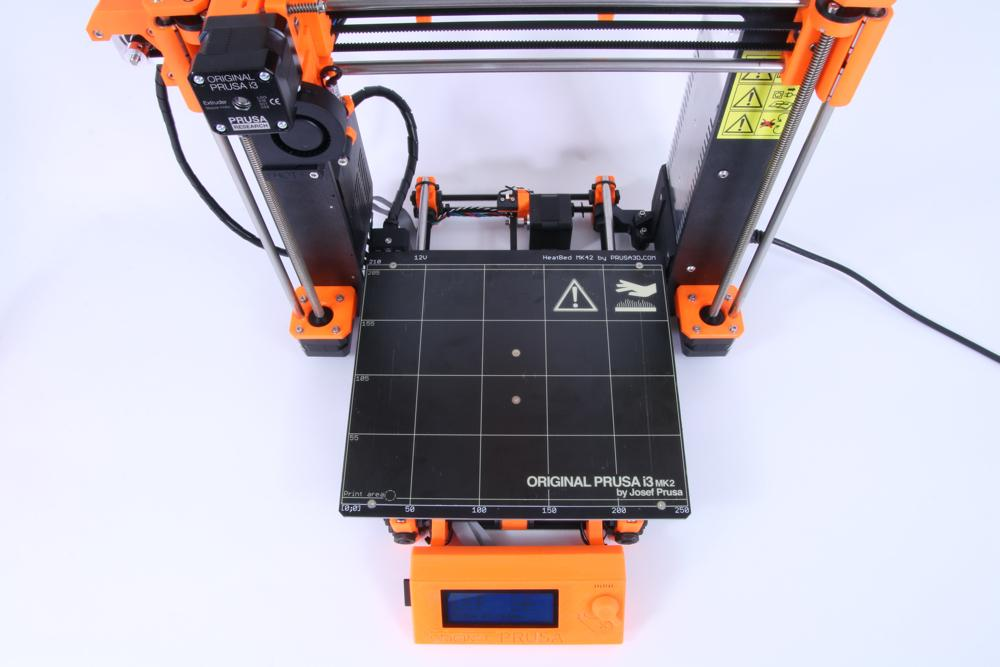
\includegraphics[ trim = {0 0 0 0}, clip , angle=0, scale=0.30 ]{imagens/prusa}
%	\caption{Prusa i3 MK2S Printer used to print the testing parts. \citep{site}}
%	\label{fig31}
%\end{figure*}



\section{METHODOLOGY}

The study consisted in 20 parts being built and tested. For these parts, the only printing parameter altered was nozzle temperature, with temperatures that ranged from 230 $^\circ C$ for parts 1 through 5 and ending with 250 $^\circ C$ for parts 16 through 20. All of them were printed in a Prusa i3 MK2S printer, using PETG XT filament from 3Dfila. They had 100\% infill and were printed in the longitudinal direction, meaning a 0 $^\circ$ angle between the layers and the heated bed. 
The test procedure was conducted in accordance to the ASTM D638-02a standard \citep{norma}, with the exception of the testing speed which was reduced from 5 mm/min to 1 mm/min to prevent issues such as the heating of the parts.
Each part was placed on an MTS Landmark 647 machine as shown in Fig.\ref{fig30} and then subjected to increasing tensile stress, being pulled on the y axis from one end while remaining fixed on the other, until rupture. The MTS software was used to gather and export the results. 

\begin{figure*}[h!]
	\centering
	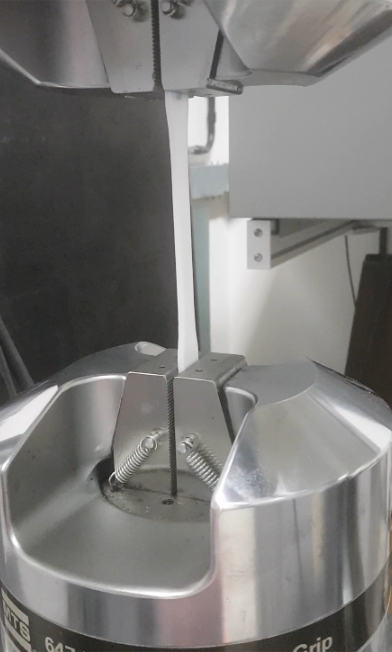
\includegraphics[ trim = {0 1cm 0 0cm}, clip , angle=0, scale=0.80 ]{imagens/maquina}
	\caption{Testing part fixed on MTS Landmark 647.}
	\label{fig30}
\end{figure*}

In the end, the results were compared with the mechanical properties of the PETG polymer from literature. 



\section{SPECIMENS}

The tensile stress testing parts were designed following the geometry specified in the ASTM D638-02a standard (Type I specimen, with 7mm thickness) as utilized on \citep{test_on_fdm}. The geometry designed can be seen on Fig.\ref{fig1}.

\begin{figure*}[h!]
	\centering
	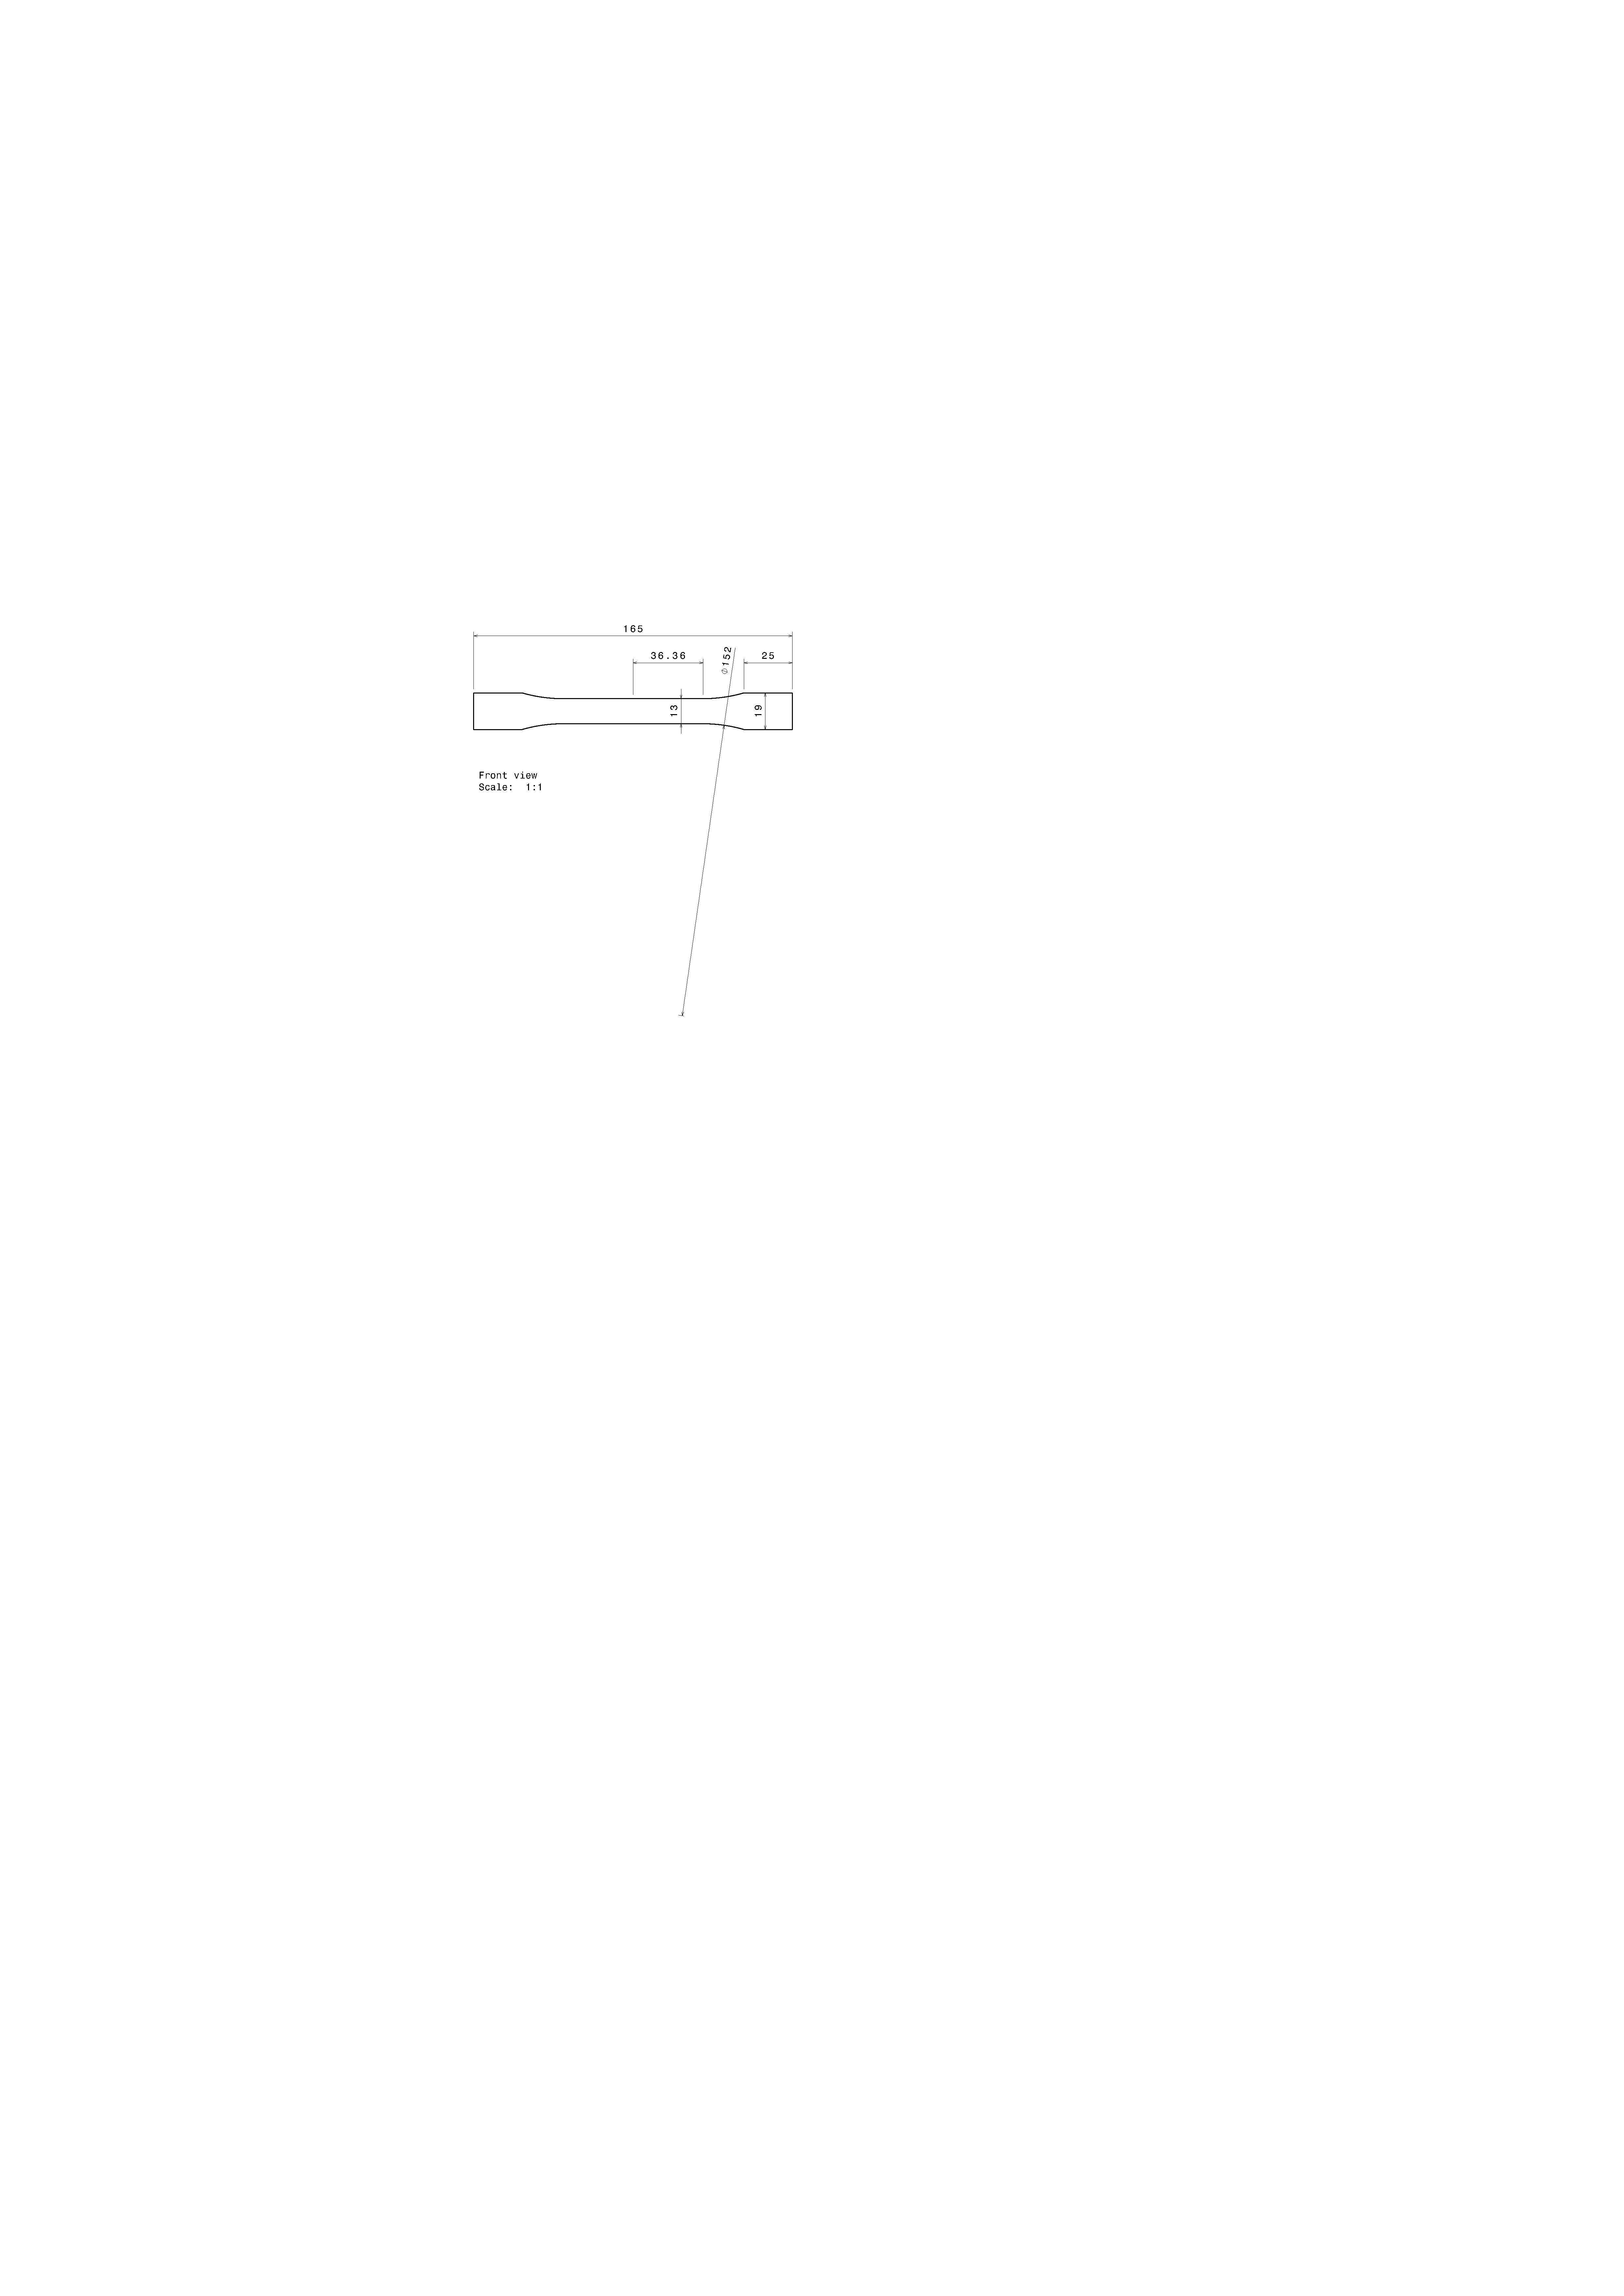
\includegraphics[ trim = {24cm 80cm 43cm 32cm}, clip , angle=0, scale=0.80 ]{imagens/Drawing1}
	\caption{Test parts CAD Draw.}
	\label{fig1}
\end{figure*}


From this sketch, a 3D model was designed on the CATIA V5 CAD software (Figure \ref{fig2}). Such model was then exported as a STL file to the slicing software (Simplify3D), as seen on Fig.\ref{fig3}.


\begin{figure*}[h!]
	\centering
	\begin{subfigure}[b]{0.5\textwidth}
		\centering
		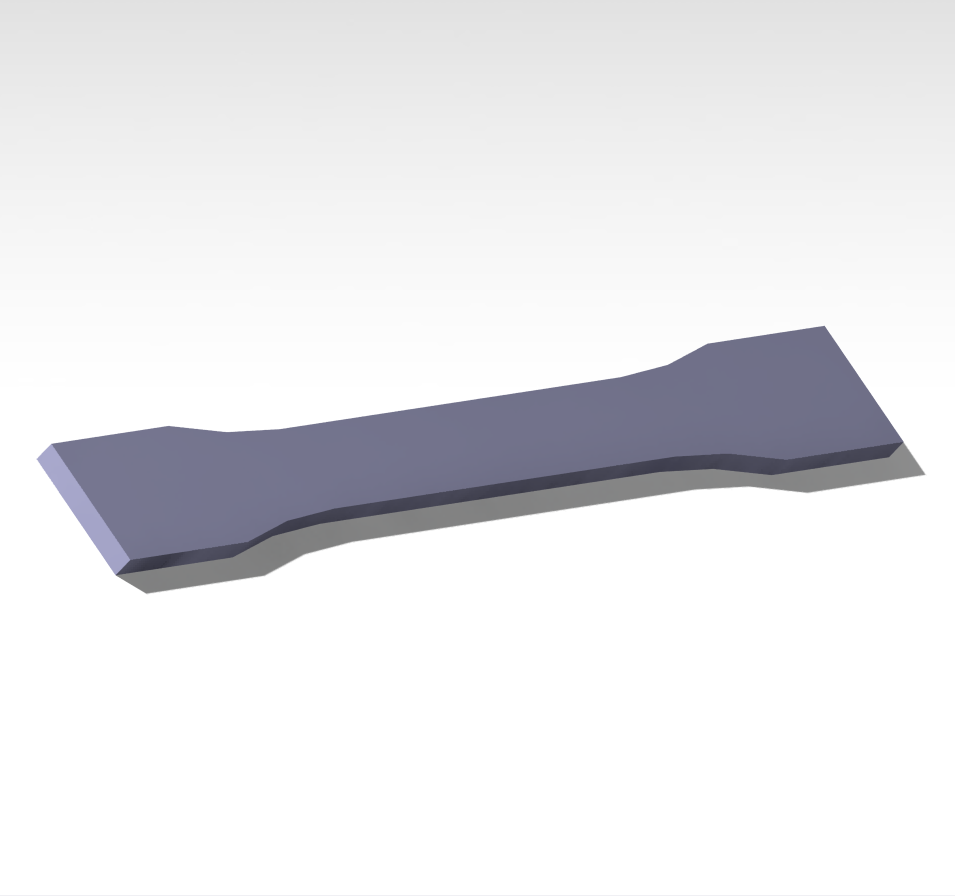
\includegraphics[ trim = {0 0 0 0}, clip , angle=0, scale=0.063 ]{imagens/renderizacao}
		\caption{CAD rendering.}
		\label{fig2}
	\end{subfigure}%
	~ 
	\begin{subfigure}[b]{0.5\textwidth}
		\centering
		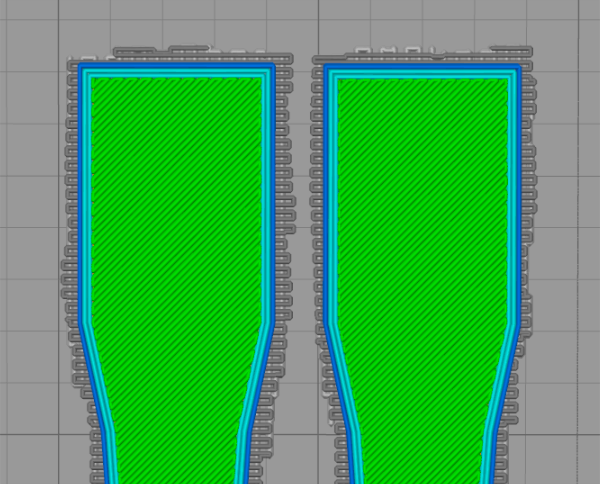
\includegraphics[ trim = {0cm 0cm 0 0cm}, clip , angle=0, scale=0.45 ]{imagens/Esboco2}
		\caption{Sliced part`s G code, made with Simplify3D software.}
		\label{fig3}
	\end{subfigure}
	\caption{Modeling and slicing of the specimen for printing.}
\end{figure*}

In Fig. \ref{fig3}, it is possible to see that the parts were made on a support bed. In other words, not directly on the heated bed. Such method is used to secure the z axis regularity of the printed parts, as the fist layer printed directly over the heated plate has very different properties from the rest of the print \citep{PETG}. 

It is important to point out the qualities that will be set constantly through all the test specimens. These parameters will not be discussed on the present paper: The Nozzle diameter was 0.4 mm, the retraction distance and speed were 5 mm and 2100 mm/min, the layer height was 0.15 mm, with 3 lateral outer layers (Fig.\ref{fig3}) and the Heated bed was set to 80 degrees Celsius.

The infill percentage was set to 100\%. The layers were made out of parallel lines and from one layer to the other the inclination of these lines varied 90 $^\circ$ from one another and made 45 $^\circ$ with the y axis of the print.









%
%\begin{table}[!h]
%\centering
%\caption{Experimental results for flexural properties of CFRC-4HS and CFRC-TWILL composites. \protect\\Span/depth ratio = 35:1. Average results of 7 specimens.}
%\begin{tabular}{|c|c|c|}
%\hline
%Composite Properties & CFRC-TWILL & CFRC-4HS\\
%\hline
%Flexural Strength (MPa)$^{(1)}$ & 209$\pm$ 10 & 180 $\pm$  15\\
%\hline
%Flexural Modulus (GPa)$^{(1)}$ & 57.0 $\pm$ 2.8 & 18.0 $\pm$  1.3\\
%\hline
%Mid-span deflection at the failure stress (mm) & 2.15 $\pm$  1.90 & 6.40 $\pm$  0.25\\
%\hline
%\end{tabular}
%\\
%\begin{tabular}{p{11cm}ll}
%$^{(1)}$ measured at 25$^{o}$C & &
%\end{tabular}
%\label{tab1}
%\end{table}



\section{RESULTS}
The data obtained from the five parts for each temperature are plotted in Fig.\ref{fig7} and linear regression was used to calculate the Young's Modulus of each part.

\begin{figure*}[h!]
	\centering
	\begin{subfigure}[b]{0.5\textwidth}
		\centering
		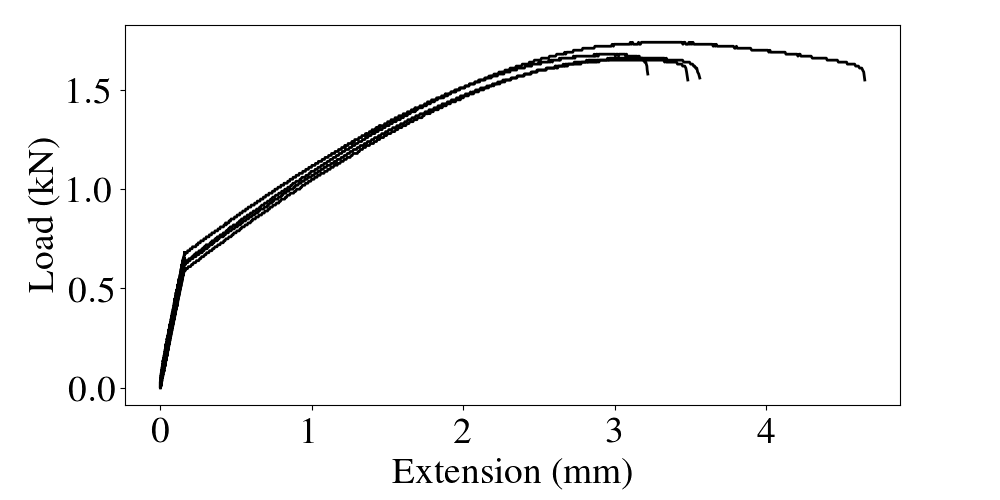
\includegraphics[ trim = {0 0 0 0}, clip , angle=0, scale=0.35 ]{imagens/230_bruto}
		\caption{Five specimens for the temperature of $230^\circ$.}
		\label{fig22}
	\end{subfigure}% 
	\begin{subfigure}[b]{0.5\textwidth}
		\centering
		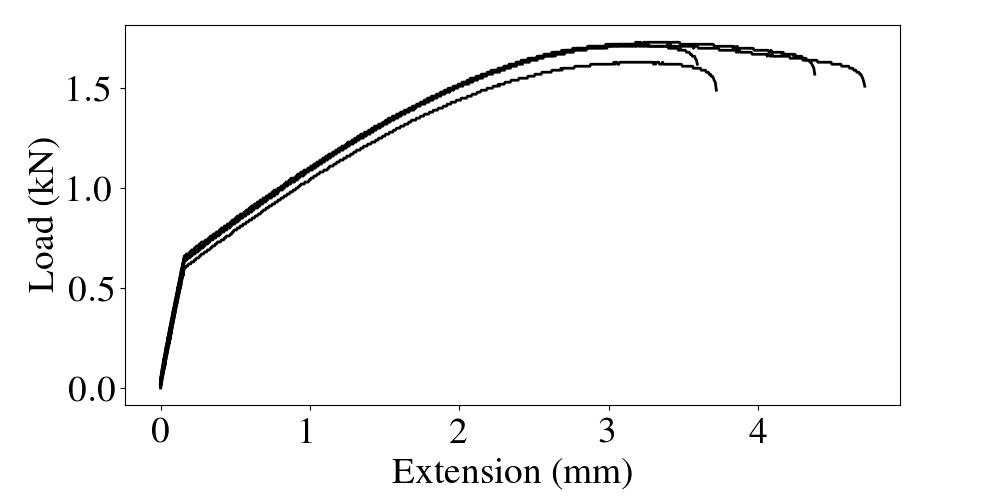
\includegraphics[ trim = {0 0 0 0}, clip , angle=0, scale=0.35 ]{imagens/240_bruto}
		\caption{Five specimens for the temperature of $240^\circ$.}
		\label{fig4}
	\end{subfigure}
\\
	\begin{subfigure}[b]{0.5\textwidth}
		\centering
		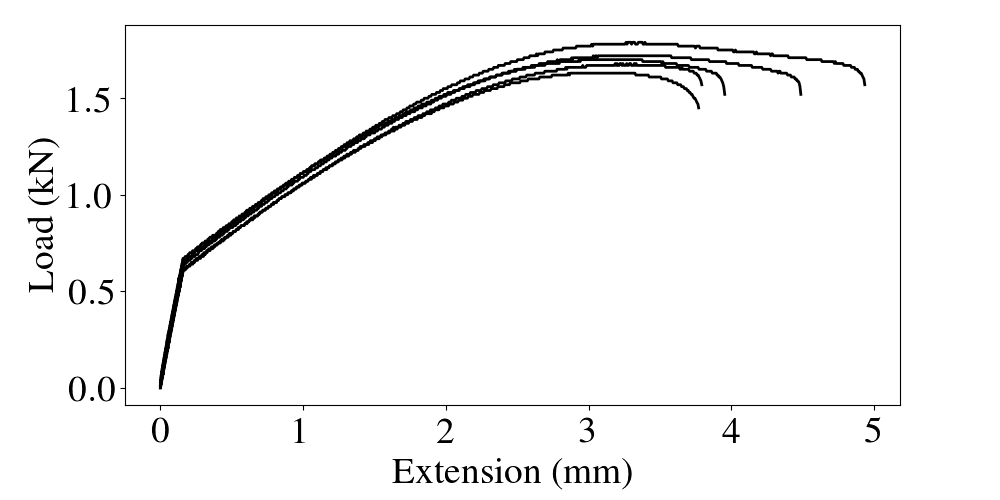
\includegraphics[ trim = {0cm 0cm 0 0cm}, clip , angle=0, scale=0.35 ]{imagens/245_bruto}
		\caption{Five specimens for the temperature of $245^\circ$.}
		\label{fig5}
	\end{subfigure}
	\begin{subfigure}[b]{0.49\textwidth}
		\centering
		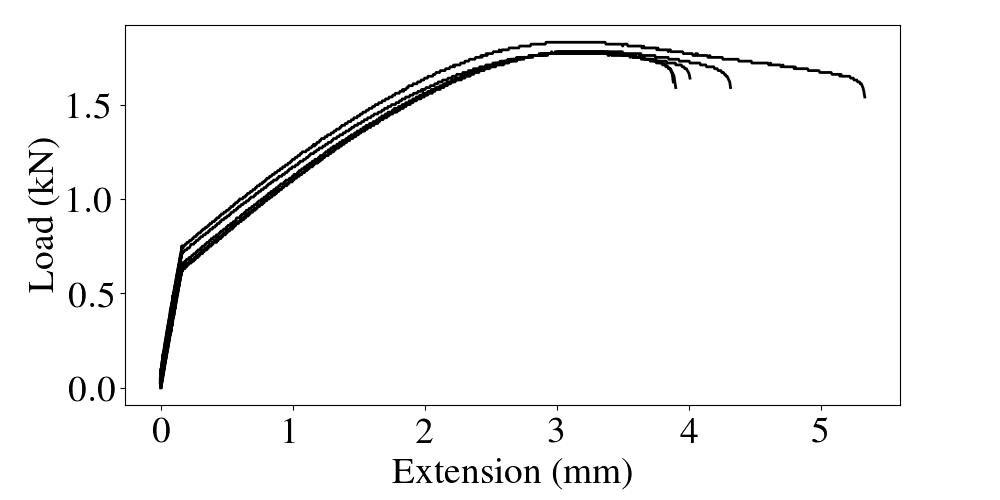
\includegraphics[ trim = {0cm 0cm 0 0cm}, clip , angle=0, scale=0.35 ]{imagens/250_bruto}
		\caption{Five specimens for the temperature of $250^\circ$.}
		\label{fig6}
	\end{subfigure}
	\caption{Tensile tests performed on each test part. Five tests for each temperature (each line is a experiment).}
	\label{fig7}
\end{figure*}
 
From Fig.\ref{fig7} it is possible to see that some regularity was achieved. The overall behavior was very steady, with similar curve profiles between the specimens, but there was a notable dissonance in terms of fracture point. The temperature that had the bigger extension before breaking were the 250 $^\circ C$ specimen (Fig.\ref{fig6}), with the part holding up with a maximum extension up to 5.213 mm.

The fractures on the specimens were consistently at a 45 $^\circ$ degree direction with the stress axis, as seen in Figure.\ref{fig9}: 

\begin{figure*}[h!]
	\centering
	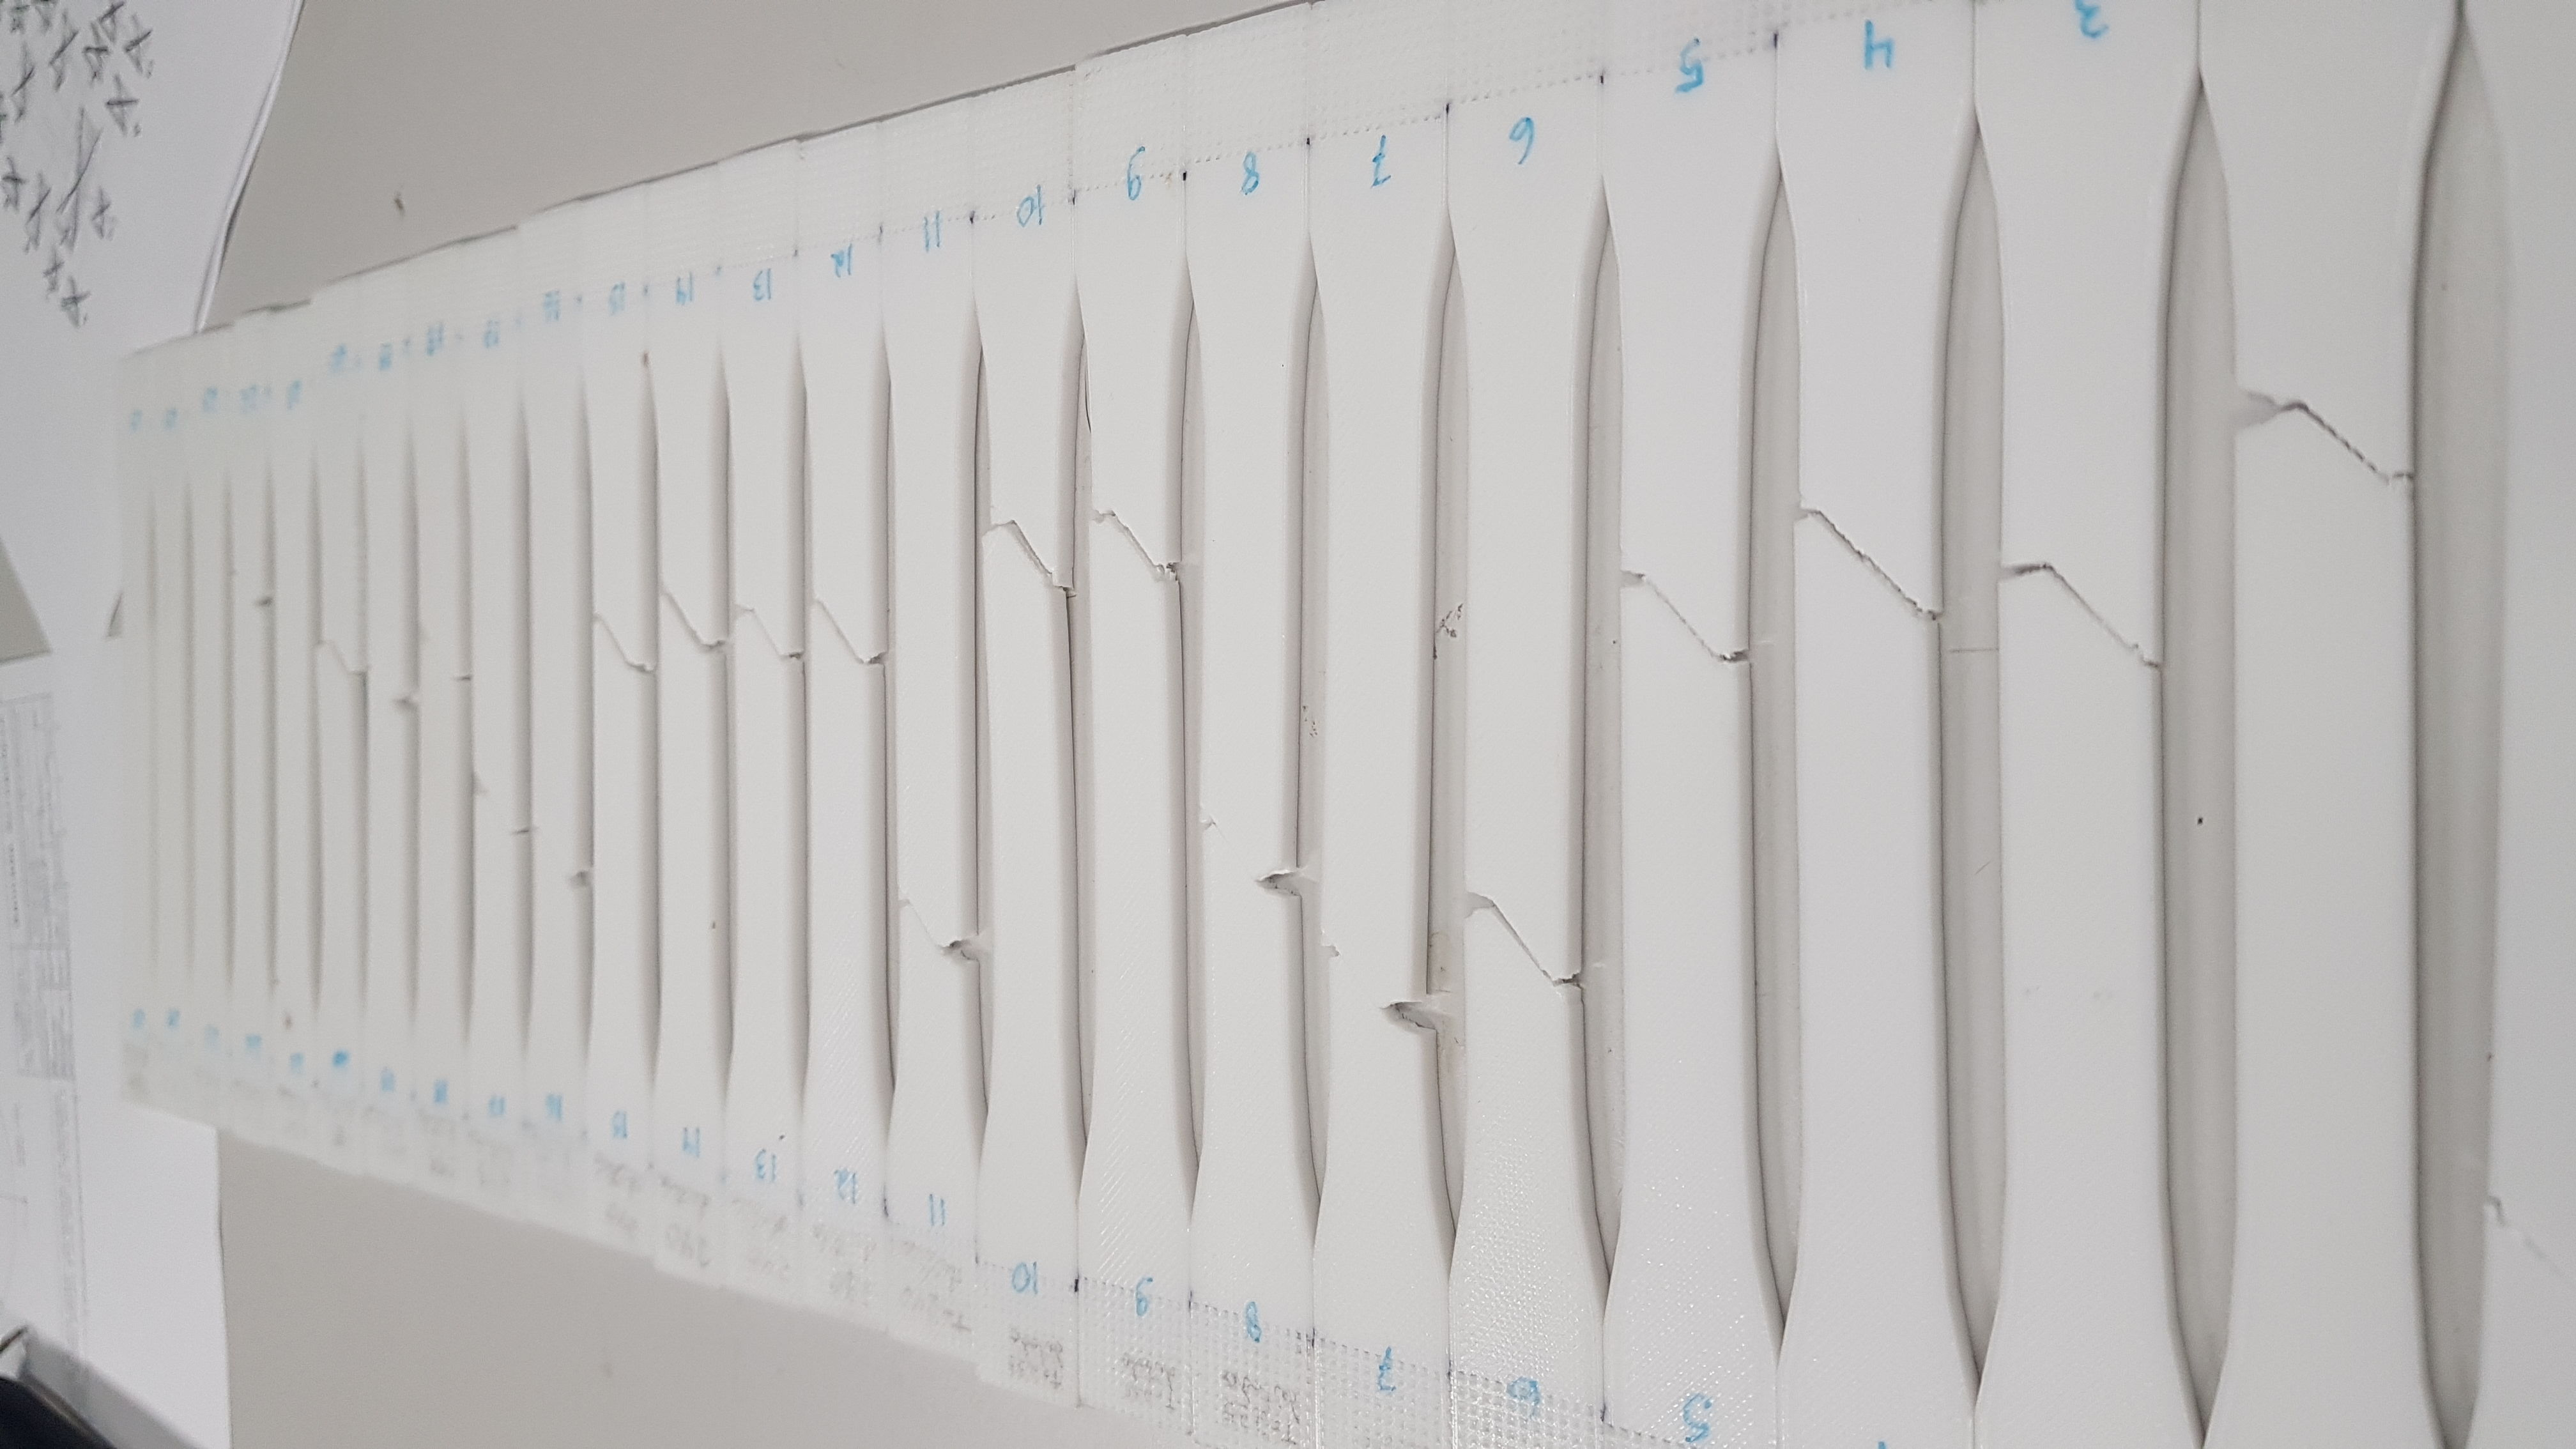
\includegraphics[ trim = {98cm 5cm 33cm 5cm}, clip , angle=90, scale=0.23 ]{imagens/fracture}
	\caption{Specimens fractured after stress test.}
	\label{fig9}
\end{figure*}

The average Young's Modulus was then calculated for each temperature, resulting in Fig.\ref{fig10}, so that their values could be better analyzed. 


\begin{figure*}[h!]
	\centering
	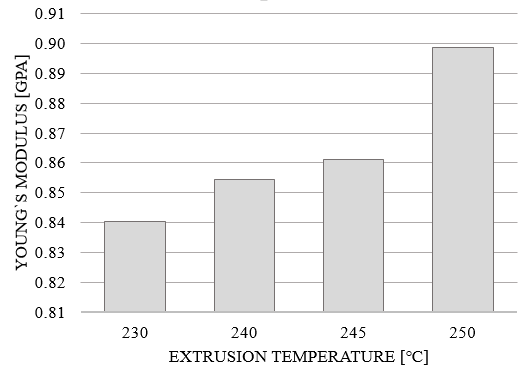
\includegraphics[ trim = {0 0 0 0}, clip , scale=0.8 ]{imagens/finais2}
	\caption{Averaged Young's modulus for each extrusion temperature.}
	\label{fig10}
\end{figure*}



The results were mostly as expected, with the Young's Modulus increasing with the increase in temperature which happens because the higher temperatures allow for better bonding between each layer of the print.

The results were close to other tests executed in literature as seen in \citep{PETG}. But in these tests the overall Young's modulus were measured around 0.7 GPa. So the results were slightly higher, possibly because diferent printing and filament qualities. 


\section{CONCLUSION}
This study shows that higher nozzle temperature results in higher Young's Modulus. Therefore, when printing mechanical parts were stress resistance is important it is better to print at higher temperatures. On the other hand, if that is not the case, it may be worth it to use lower temperatures to get a better superficial finishing in the printed part, as lower temperatures prevent warping and stringing. 








\section{ACKNOWLEDGEMENTS}
The authors would like to thank the following professors and institutions: Dr. Ruham Pablo Reis, Dr. Pedro Pio Rosa Nishida, Lmest (Structural Mechanics Laboratory), FEMEC (Mechanical engineering College), UFU (Federal University of Uberl\^andia) and, especially, EPTA (Propulsion and Aerospace Technology Team) for financial and technical support.




\section{REFERENCES} 

\bibliographystyle{abcm}
\renewcommand{\refname}{}
\bibliography{bibfile}

\end{document}
